\subsection{Mediterranean Sea (2003)}

During 2003 the Mediterranean Sea saw it's largest event recorded, being on average $4^{\circ}$C for 30 days, from this event saw mass mortality of marine life in the surrounding rocky reefs.

\begin{figure}[H]
\centering
    \textbf{-37$^{\circ}$N 287$^{\circ}$E}\par
    \makebox[\textwidth][c]{
        \includegraphics[width=0.75\textwidth, angle =0]{Chapter3/ArabianSea/MS.png}
        }
            \caption{A figure of SST at 40$^{\circ}$N 06$^{\circ}$E between January 2012 - January 2013. Recorded temperatures are indicated by the black line, expected temperatures (climatology) is indicated by the blue dashed line and 90th percentile temperatures are indicated by the red dotted line. Hence, the filled colour area indicates MHW days, where the darker the shade, the higher the intensity of the MHW. \cite{MHWtracker}}
            \label{fig:MS}
\end{figure}

Looking at figure \autoref{fig:MS}, we can see the MHW starts around the start of June and continues till around the middle of September.  
\\\\
Again to investigate the impacts this MWH may of had on the health of phytoplankton we will produce a ARIMA model using our chlorophyll concentration data and compare it to our recorded data and try to find any anomalies that may have been caused by the abnormally high SST.
\\\\
Looking at \autoref{fig:MSts}, we can see that the chlorophyll concentration is mostly lower than what would be expected from our ARIMA model. This is in accordance with what we would expect due to the lower availability of nutrients for the phytoplankton to consume in warm water.

\begin{figure}[H]
\centering
    \textbf{40$^{\circ}$N 06$^{\circ}$E}\par
    \makebox[\textwidth][c]{
        \includegraphics[width=0.5\textwidth, angle =-90]{Chapter3/ArabianSea/Data_40N6E_Chl_TS.eps}
        }
            \caption{A figure of our ARIMA model calculated using our chlorophyll data set and our raw data for 40$^{\circ}$N 06$^{\circ}$E}
            \label{fig:MSts}
\end{figure}